  
\documentclass[12pt,a4paper,fleqn]{tufte-handout} 
\usepackage{graphicx} 
\usepackage{morefloats} 
\usepackage{amsmath} 
\usepackage{amssymb} 
\usepackage{rotating} 
% mcode options for matlab code insertion bw (for printing), numbered (line numbers), framed (frame around code blocks), useliterate (convert Matlab expressions to Latex ones), autolinebreaks (automatic code wraping, use it with caution 
\usepackage[literate]{mcode} 
\graphicspath{{figures/}{tex}{../figures/}{../../}{../}}  
\title[clustering]{clusteringDemonstration} 
\author{ Mathieu Lagrange } 
  
\begin{document} 
  
\maketitle 
  
\section{Introduction}


This document documents the first demonstration of the use of the expLanes framework to conduct a computational experiment. The project clusteringDemonstration is about the comparison of several algorithms that clusters synthetic data.

\section{Design}

\begin{marginfigure}
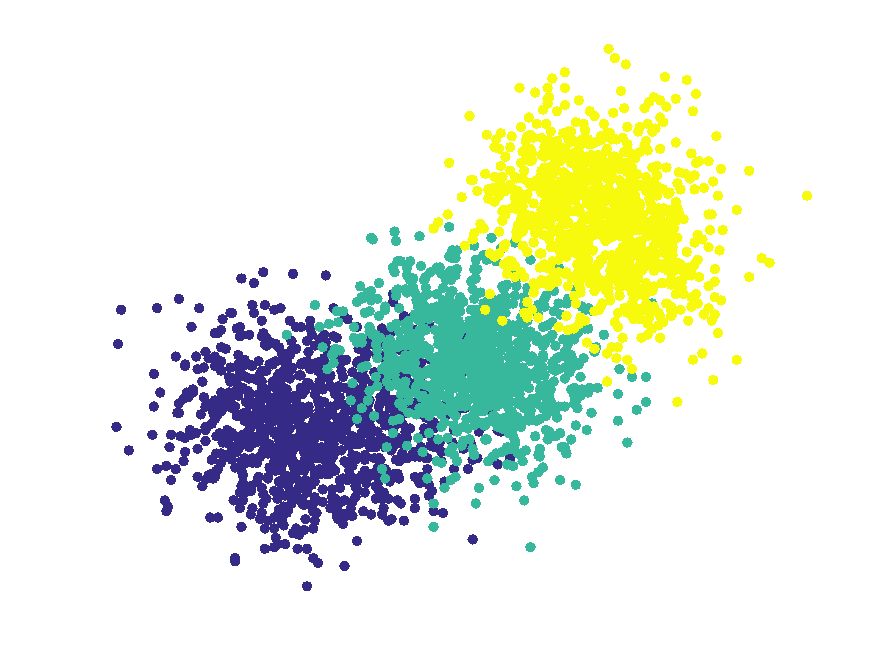
\includegraphics[width=\textwidth]{figures/scatter1}
\caption{A dataset with spiral shaped clusters.}
\label{scatter}
\end{marginfigure}

\begin{marginfigure}
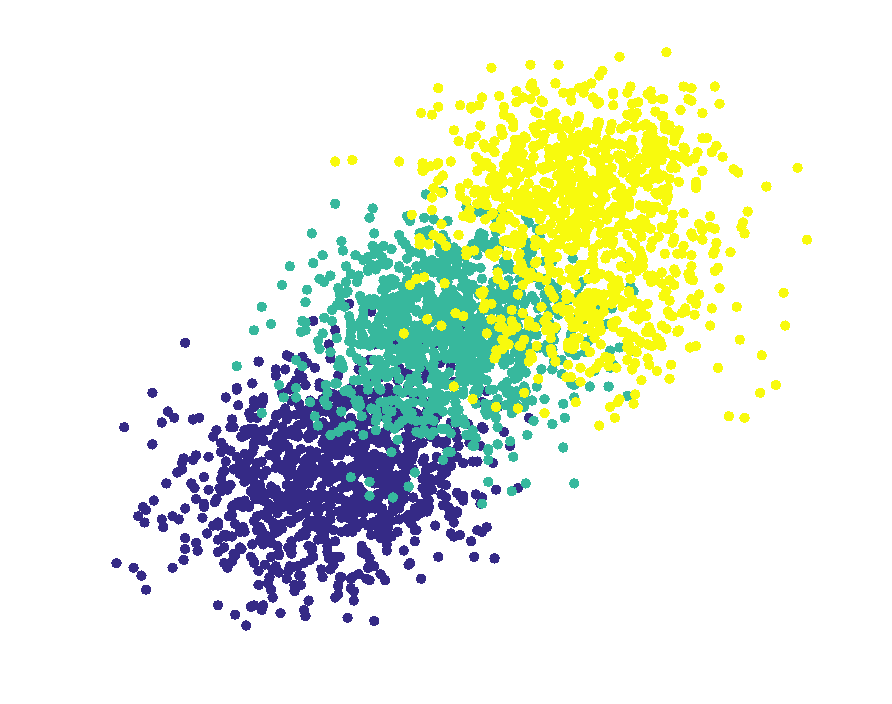
\includegraphics[width=\textwidth]{figures/scatter2}
\caption{A dataset with spherical clusters.}
\label{scatter}
\end{marginfigure}

\begin{marginfigure}
\includegraphics[width=\textwidth]{figures/scatter3}
\caption{A dataset with Gaussian clusters.}
\label{scatter}
\end{marginfigure}

 The project is divided into two processing steps:
\begin{enumerate}
\item \textbf{generate}: generation of the synthetic datasets
\item \textbf{compute}: clustering of those datasets and comparison of the resulting clustering with true ones using standard performance metrics
\end{enumerate}

\subsection{\textbf{Generate step}: generation of synthetic datasets}



Each dataset comprises a set of points in a 2D space. Those points are grouped into classes of different shapes. The factors of variability that are to be tested are:
\begin{itemize}
\item the number of classes
\item the shape of each clusters: spherical, spiral, and Gaussian
\item the number of data points per class.
\end{itemize}

This step outputs for each dataset the location of the data points (elements) as well as the class to which they belong to (class).

\subsection{\textbf{Compute step}: Computation of distances}

Once the datasets are generated, the data can be clustered into a predefined number of clusters using several algorithms. The main factor for this step is then the type of clustering algorithm. We consider three algorithms, the well known kMeans algorithm\cite{macQueenBsmsp67}, the kernel kMeans one\cite{Girolami}, and the kMedoids one\cite{Kaufman1987}.

For the kernel kMeans algorithm, one needs to specify the type of kernel, and for the exponential kernel, the $\sigma$ has to be set. For the kMedoids algorithm, the type of similarity has to be specified. In order to have a lower bound baseline, the \mcode{chance} method is considered as a random placement of the elements into the clusters.

For all the algorithms, the clustering is run several times and the clustering with lowest intra-class distance is selected. Then, this process is run several times to gain statistical confidence in the observations by considering different initializations.

\subsection{Observations}

We consider the following metrics:
\begin{enumerate}
\item \textbf{accuracy}: accuracy between the reference clustering and the achieved clustering maximally aligned with the reference clustering.
\item \textbf{nmi}: normalized mutual information
\end{enumerate}

\section{Definition of factors}

Those factors and their corresponding modalities are defined in the file named \texttt{cldeFactors.txt} whose content is the following:
\lstinputlisting{../cldeFactors.txt}

Please note the \mcode{2/2} between the last two equals of the factor definition of factor \mcode{kernel} which specify that this factor is needed only for the second modality of the third factor \mcode{method}. Along the same line, the \mcode{1/0/1,1/[2 3]/2} between the last two equals of the factor definition of factor \mcode{nbClasses}  specify that its first modality is relevant for all the modalities of the factor \mcode{dataType}, but its second modality is relevant only for the second and third modalities of the factor \mcode{dataType}. Most the factor design discussed above is compactly displayed in Figure \ref{factorFlowGraph}.

\begin{figure}
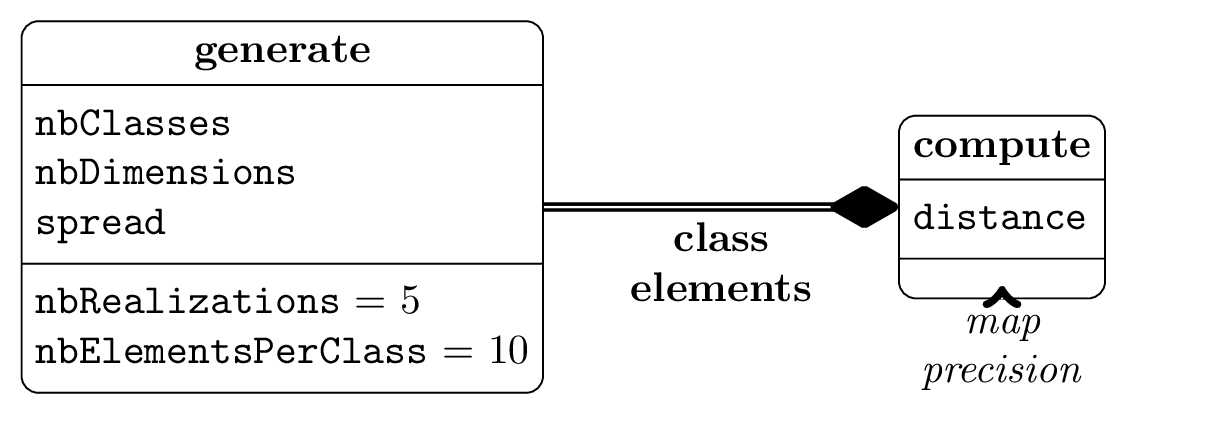
\includegraphics[width=\textwidth]{figures/factors}
\caption{Factor and data flow graph.}
\label{factorFlowGraph}
\end{figure}

\section{Results}

The results discussed next are generated as follows:
\lstinputlisting[firstline=11, lastline=14]{../cldeReport.m}

\subsection{Gaussian clusters}

Gaussian shaped clusters are notoriously easy, so the performance are quite good for this dataset, see Table \ref{dattypgauNbcla2}. In this case, the kMeans and the kernel kMeans algorithm with linear, polynomial and exponential kernels generates equivalent clustering solutions.

\subsection{Spherical clusters}

The spherical shaped clusters are not linearly separable, thus the kMeans produces results that are close to chance, see Table \ref{dattypsphNbcla2}. The kMedoids approach does not help either, as for the kernelKmeans with linear and polynomial kernel. Only an exponential kernel with a rather specific $\sigma$ value is able to increase the performance above chance.

\subsection{Spiral shaped clusters}

The spiral shaped clusters are also not linearly separable. The same conclusions can be drawn, expect that the choice of the $\sigma$ value appears as less critical, see Table \ref{dattypspiNbcla2}.


\begin{marginfigure}
\includegraphics[width=\textwidth]{figures/clustering}
\caption{Clustering of the spiral shaped dataset using the exponential kernel.}
\label{clustering}
\end{marginfigure}

Concerning the observations metrics, the accuracy is an interesting metric as it relates directly to the task at hand. That said, it has to be compared to the chance baseline in order to reduce the impact of the topology of the dataset considered. In this respect, the nmi is an interesting alternative that appears to be, for those simple datasets, well correlated with the accuracy, while being less influenced by the topology of the dataset.

\subsection{Computation time}

The average computation time for the different clustering methods can be displayed using:
\lstinputlisting[firstline=16, lastline=17]{../cldeReport.m}
The results shown on Table \ref{all} reflect well the ranking of the different methods in terms of computational complexity.


\input{tex/exposeTmp} % expLanesInsertionFlag DO NOT CLEAR (but move it where you want the generated temporary LaTEX code to be inserted) 
  
  
\bibliographystyle{abbrvnat} 
\bibliography{bib} 
  
\end{document} 
